
\subsection{Steady Growth}

  \begin{figure}[h]
    \begin{center}
      
\includegraphics[width=0.3\textwidth]{img/steady200.eps}
    \end{center}
    \caption{Polygon mit 200 Punkten (Steady Growth)}
    \label{fig:steady200}
  \end{figure}

  \enquote{Steady Growth} ist einer der mehreren im Paper~\cite{held98polygons}
  beschriebenen Algorithmen zur Generierung von einfachen Polygonen.

  \enquote{Steady Growth} konstruiert ein einfaches Polygon in dem er in jeder
  Iteration einen neuen Punkt zu dem Polygon hinzuf"ugt, wobei der Punkt mit
  bestimmten Einschr"ankungen gew"ahlt werden muss, so dass das Polygon in jeder
  Iteration einfach bleibt.

  \subsubsection{Algorithmus}

\begin{code}[caption={Steady Growth}, mathescape=true]
$P_0$ $\leftarrow$ choose random triangle such that no remaining points are inside of this triangle
$S_0$ $\leftarrow$ $S_0$ $\setminus$ $P_0$

for i = 1 to n - 3 do
  repeat
    $s_i$ $\leftarrow$ choose random point in $S_{i-1}$
    $\CH_i$ $\leftarrow$ construct the convex hull of $P_i$ $\cup$ $\{s_i\}$
  until $\CH_i$ contains no point of $S_{i-1}$ $\setminus \{s_i\}$

  $S_i$ $\leftarrow$ $S_{i-1}$ $\setminus$ $\{s_i\}$

  ($v_k$, $v_{k+1}$) $\leftarrow$ find an edge in the Polygon $P_{i-1}$ that is completely visible from $s_i$
  $P_{i+1}$ $\leftarrow$ replace the edge ($v_k$, $v_{k+1}$) by the edges ($v_k$, $s_i$) and ($s_i$, $v_{k+1}$)

\end{code}

    Wobei $S_i$ die Punktmenge, $P_i$ das Polygon und $\CH_i$ die Konvexe H"ulle
    in der $i$-ten Iteration ist.

    Als erstes gehen wir auf die Konvexe H"ulle ein, da diese in diesem
    Algorithmus viel benutzt wird. In \enquote{Steady Growth} wird die Konvexe
    H"ulle in jeder Iteration um einen Punkt erweitert, so dass sich eine
    Insertion Hull mit den Laufzeiten $\bigO(\log n)$ f"ur den Neuaufbau und
    $\bigO(\log n)$ f"ur den Test, ob ein Punkt in der Konvexen H"ulle liegt,
    anbieten w"urde. Dennoch haben wir die Konvexen H"ulle basierend auf Graham
    Scan implementiert, wo sich die Laufzeit f"ur den Test \enquote{Punkt in der
    Konvexen H"ulle} und der Neuaufbau der Konvexen H"ulle jeweils auf
    $\bigO(n)$ belaufen. Wir haben den einfacheren Ansatz beibehalten, da sich
    in den empirischen Tests (siehe Laufzeit) gezeigt hatte, dass die
    Konstruktion der Konvexen H"ulle kein optimierungsw"urdiger Faktor ist.

    Nun zum Finden des Startdreiecks, welches keine anderen Punkte beinhalten
    darf. In unserer urspr"unglichen Version wurden drei Punkte zuf"allig
    gew"ahlt und auf diese Eigenschaft getestet, so dass es theoretisch m"oglich
    war, dass der Algorithmus nie terminiert. Da das suchen des Startdreiecks
    bei gr"o"seren Punktmengen bemerkbar lange dauerte, haben wir folgenden
    Ansatz umgesetzt. Wir w"ahlen initial zwei Punkte $a, b$ zuf"allig, die dann
    fixiert bleiben und nehmen einen dritten Punkt $c$ hinzu. Wir bestimmen alle
    Punkte, die in dem Dreieck $\triangle(a,b,c)$ liegen. Wenn keine Punkte in
    diesem Dreieck liegen, dann wird das Dreieck gew"ahlt. Wenn nicht, dann wird
    ein neuer dritter Punkt $c$ aus den im Dreieck befindlichen Punkten gew"ahlt
    und der Vorgang wiederholt.

    Als n"achstes gehen wir auf das finden von $s_i$ ein. In unserer
    urspr"unglichen Version wurde immer ein zuf"alliger Punkt als $s_i$ gew"ahlt
    und "uberpr"uft, ob ein Punkt in der Konvexen H"ulle $\CH(P_i \cup \{s_i\})$
    liegt. Um diesen Vorgang deterministisch zu machen, wurden die schon
    probierten Punkte ge\emph{blacklist}ed.

    Danach unterlief diese Version einige Optimierungen. Als erstes wurde wie im
    Initialisierungsschritt $s_i$ zuf"allig gew"ahlt und alle in der Konvexen
    H"ulle $\CH(P_i \cup \{s_i\})$ befindlichen Punkte gesammelt. Wenn keine
    Punkte in dieser Konvexen H"ulle liegen, dann wird $s_i$ genommen. Ansonsten
    wird ein Punkt aus den gesammelten Punkten gew"ahlt und der Vorgang
    wiederholt.
    \begin{wrapfigure}{l}{0.4\textwidth}
      \vspace{-20pt}
      \begin{center}
        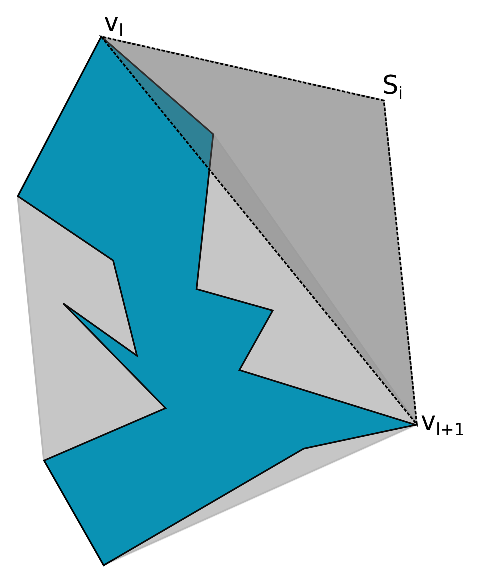
\includegraphics[width=0.38\textwidth]{img/steadyTriangle.eps}
      \end{center}
      \vspace{-20pt}
      \caption{Dreieckspunkttest}
      \vspace{-10pt}
      \label{fig:steadyTraingle}
    \end{wrapfigure}
    Der Test, ob ein Punkt in der Konvexen H"ulle liegt, dauerte
    nach dieser Optimierung immer noch im worst-case $\bigO(n)$, dass konnte
    aber auf $\bigO(1)$ verbessert werden, aufgrund folgender Eigenschaft:

    Man beachte, dass in jeder Iteration $\CH(P_{i}) \cap S_i = \emptyset$ gilt.
    Damit befindet sich jedes neue $s_i$ au"serhalb der Konvexen H"ulle des
    Polygons. Wenn ein $s_i$ gew"ahlt und die neuen Konvexe H"ulle konstruiert
    wurde, dann bilden in der neuen Konvexen H"ulle die Eckpunkte $v_l$,
    $v_{l+1}$ vor und nach $s_i$ mit $s_i$ ein Dreieck $\triangle(v_l, s_i,
    v_{l+1})$. Da jeder Punkt aus der Punktmenge $S_i$ au"serhalb der alten
    Konvexen H"ulle liegt und uns nur diejenigen Punkte aus $S_i$ interessieren,
    die innerhalb der neuen konvexen H"ulle liegen, reicht es die Anfrage auf
    den Schnitt der beiden konvexen H"ullen zu konzentrieren. Da das Dreieck
    $\triangle(v_l, s_i, v_{l+1})$ diesen Schnitt komplett beinhaltet, kann die
    Anfrage auf dieses Dreieck weiter begrenzt werden.

    Nach~\cite{held98polygons} existiert immer eine vom Punkt $s_i$ aus
    sichtbare Kante im Polygon $P_i$. N"ahrere Details zur Implementierung diese
    Abschnittes des Algorithmus ist in der Laufzeitanalyse beschrieben.

  \subsubsection{Laufzeit}

    Nach dem Paper ist die Laufzeit $\bigO(n^2)$. Im Paper kostet pro
    Schleifendurchlauf das Berechnen der sichtbaren Kanten von dem gew"ahlten
    Punkt $s_i$ $\bigO(n)$. Das finden des Punktes $s_i$ soll auch in $\bigO(n)$
    m"oglich sein, leider wurde nicht angegeben, wie man einen passenden Punkt
    $s_i$ in $\bigO(n)$ finden kann, der trotzdem zuf"allig ist.

    In unserer Implementierung braucht das Suchen nach $s_i$ im worst-case
    $\bigO(n^2)$, wenn in jeder Iteration nur ein Punkt rausgenommen wird. Der
    Test, ob ein Punkt in der erweiterten Konvexen H"ulle liegt, ist aufgrund
    der obigen Beobachtung in $\bigO(1)$ m"oglich (Punkt in Dreieck). Wenn in
    jedem Schritt ungef"ahr die H"alfte der Punkte eliminiert werden, dann
    kommen wir auf eine Laufzeit von $\bigO(n)$. Dies lies sich auch empirisch
    bei 100 Durchl"aufen mit je 1000 Punkten best"atigen. Durchschnittlich waren
    2 bis 3 Iterationen und in allen Durchl"aufen maximal 10 Iterationen
    notwendig, um $s_i$ zu finden. Bei gr"o"seren Punktmengen (2000, 3000, 4000)
    ergaben mit weniger Durchl"aufen ($10$ bis $20$) "ahnliche Ergebnisse
    (durchschnittlich 2 bis 3 Iterationen, maximal 12 Iterationen).
    Durchschnittlich dauerte das Suchen nach $s_i$ bei 1000 Punkten
    $0.100$\footnote{Messwerte auf einem Intel Atom N450 mit 1.66Ghz ermittelt}
    bis $0.180$ms und bei 2000 Punkte $0.150$ bis $0.200$ ms. Wie oben schon
    beschrieben, haben wir auf Optimierungen nach der Suche von $s_i$
    verzichtet, obwohl dies m"oglich ist.

    Das Suchen nach der sichtbaren Kante dauerte empirisch deutlich l"anger.
    Dies ist weiter nicht Verwunderlich, da wir eine einfache Implementierung
    f"ur das finden einer von $s_i$ sichtbaren Kante haben. Wir gehen jeden
    Eckpunkt des Polygons durch, bis zwei aufeinander folgende Eckpunkte $v_k,
    v_{k+1}$ von $s_i$ sichtbar sind. Daf"ur schneiden wir das Polygon mit der
    Strecke $\overline{s_i v_k}$. Das dauert bei uns $\bigO(n)$, womit insgesamt
    $\bigO(n^2)$ Zeit ben"otig wird, um die Kante zu finden. Durchschnittlich
    dauerte das Suchen nach der sichtbaren Kante bei 1000 Punkten $120$ bis
    $150$ ms und bei 2000 Punkten $233$ bis $343$ ms. Damit besitzt der
    Algorithmus hier Optimierungspotenzial.

    Somit braucht unsere Implementierung von \enquote{Steady Growth}
    $\bigO(n^3)$ Zeit.

  \subsubsection{Eigenschaften}

    Da \enquote{Steady Growth} von innen nach au"sen w"achst, sind in dem
    resultierenden Polygon viele Verzweigungen und Verwindungen. Mittelgro"se
    Punktmengen mit 1000 bis 2000 Punkten sind in vertretbarer Zeit generierbar.
    Und die Punkte des erzeugten Polygon sind in CCW angeordnet. Im Paper
    \cite{held98polygons} wird angemerkt, dass \enquote{Steady Growth} nicht
    jedes m"ogliche Polygon erzeugen kann.
